\chapter{弦与杆中的波：达朗贝尔方程}\label{ch:b2:waves-on-strings}

拨动吉他弦，一个波形沿弦传播，并在
琴桥处反射、折返，最终形成驻波图样，
其频率即为你听到的音高。把耳朵贴近铁轨，
列车尚未到达时你便已听见它：一道压缩波以
每秒五千米的速度沿钢轨传来。本科一年级分册描述过这类
波——行波、驻波与叠加波——却未说明它们为何存在。
本章导出支配它们的方程，
\emph{达朗贝尔波动方程}，先讨论弦的横向运动，
再讨论由质点与弹簧逐个原子搭建而成的杆的纵向运动；
并计算波携带的能量，
以及波遇到介质变化时决定其行为的阻抗。

\section{弦的振动}

\begin{theorem}[弦的波动方程]\label{thm:b2:waves-on-strings:equation}
\index{达朗贝尔方程}\index{波动方程}\index{波速（弦）}
线密度为 $\mu$、张紧于张力 $T$ 之下的弦，
发生微小横向位移 $y(x, t)$（斜率 $|\partial_xy| \ll 1$）。则
\[
\frac{\partial^2y}{\partial t^2} = c^2\,\frac{\partial^2y}{\partial x^2} ,
\qquad c = \sqrt{\frac{T}{\mu}} ,
\]
此即\emph{达朗贝尔方程}，其通解为 $y = f(x - ct)
+ g(x + ct)$：向右与向左以速率 $c$ 传播的两个波形的叠加，
二者均保持形状不变。
\end{theorem}

\begin{proof}
取位于 $x$ 与 $x + \dd x$ 之间、质量为 $\mu\,\dd x$ 的弦元。其
两侧邻近部分以张力 $T$ 沿切线方向拉动它：
水平方向两端均为 $T\cos\theta \approx T$（水平方向无运动，故
$T$ 处处相同），竖直方向为 $T\sin\theta \approx T\partial_xy$，由此
得合力 $T[\partial_xy(x + \dd x) - \partial_xy(x)] = T\,\partial_x^2y\,\dd x$。
由牛顿第二定律，$\mu\,\dd x\,\partial_t^2y = T\partial_x^2y\,\dd x$。为求解，令
$u = x - ct$，$v = x + ct$，方程化为 $\partial_u\partial_vy = 0$，
由链式法则，故 $\partial_vy$ 仅依赖于 $v$，于是 $y = f(u) + g(v)$；
反之，任何这样的 $y$ 均满足该方程。重力可略去，
当 $T \gg \mu gL$ 时则是合理的。
\end{proof}

\begin{omfigure}
\begin{tikzpicture}[font=\small, x=1cm, y=1cm, >=Stealth]
  \begin{scope}
    \draw[->] (-2.5,0) -- (3.0,0) node[right, font=\footnotesize] {$x$};
    \draw[omDef, very thick, domain=-2.3:2.8, samples=60] plot (\x,{0.9*exp(-(\x)^2/1.6)});
    \coordinate (A) at (-0.6,{0.9*exp(-0.36/1.6)}); \coordinate (B) at (0.2,{0.9*exp(-0.04/1.6)});
    \fill[omThm] (A) circle (1.5pt); \fill[omThm] (B) circle (1.5pt);
    \draw[omThm, very thick, ->] (A) -- ($(A)+(-0.9,-0.55)$) node[above left, font=\footnotesize, yshift=2pt] {$\vect T(x)$};
    \draw[omThm, very thick, ->] (B) -- ($(B)+(1.0,-0.12)$) node[right, font=\footnotesize] {$\vect T(x+\dd x)$};
    \draw[dashed] (-0.6,0) -- (A); \draw[dashed] (0.2,0) -- (B);
    \node[font=\footnotesize] at (-0.6,-0.3) {$x$}; \node[font=\footnotesize] at (0.35,-0.3) {$x + \dd x$};
    \node[font=\footnotesize] at (0.2,-0.9) {$\mu\,\dd x\,\partial_t^2y = T\,\partial_x^2y\,\dd x$};
  \end{scope}
  \begin{scope}[xshift=7.6cm]
    \draw[->] (-2.5,0) -- (3.0,0) node[right, font=\footnotesize] {$x$};
    \draw[omDef, thick, domain=-2.3:2.8, samples=60] plot (\x,{0.8*exp(-(\x+1.3)^2/0.5)});
    \draw[omDef, thick, dashed, domain=-2.3:2.8, samples=60] plot (\x,{0.8*exp(-(\x-0.5)^2/0.5)});
    \draw[omDef, thick, ->] (-1.0,1.0) -- (0.2,1.0) node[above, font=\footnotesize, pos=0.5] {$c$};
    \node[font=\footnotesize] at (-1.3,-0.35) {$t$}; \node[font=\footnotesize] at (0.5,-0.35) {$t + \tau$};
    \node[font=\footnotesize] at (0.2,-0.9) {$y = f(x - ct)$};
  \end{scope}
\end{tikzpicture}

{\small 左：弦元所受的力——弦弯曲时两端张力
不再平行，其合力沿横向。
右：形状 $f(x - ct)$ 以速率 $c$ 向右传播，
且不变形。}
\end{omfigure}

\begin{example}[吉他、钢琴与电缆]\label{ex:b2:waves-on-strings:numbers}
吉他的低音 E 弦（$\mu = \qty{5.5}{g/m}$，长 \qty{0.65}{m}，
\qty{82.4}{Hz}）以基音振动，此时 $\lambda = 2L$，$c = 2Lf =
\qty{107}{m/s}$，且 $T = \mu c^2 = \qty{63}{N}$。钢琴的 A$_4$ 弦（钢质，
\qty{1}{mm}，$\mu = \qty{6.1}{g/m}$，长 \qty{0.38}{m}，\qty{440}{Hz}）：$c = \qty{334}{m/s}$，
$T = \qty{680}{N}$——钢琴中约有 $230$ 根弦，二十
吨的张力施加于铸铁框架。一根 \qty{1}{kg/m} 的电缆，
张力为 \qty{10}{kN} 时，波速为 \qty{100}{m/s}。
\end{example}

\section{驻波与简正模}

\begin{proposition}[两端固定弦的简正模]\label{prop:b2:waves-on-strings:modes}
\index{简正模}\index{谐音}\index{驻波}
两端固定于 $x = 0$ 与 $x = L$ 处的弦，存在正弦驻波解
（\emph{简正模}）
\[
y_n(x, t) = A_n\sin\frac{n\pi x}{L}\cos(\omega_nt - \varphi_n) , \qquad
f_n = \frac{\omega_n}{2\pi} = n\,\frac{c}{2L} = n f_1 , \quad n = 1, 2, 3, \dots
\]
——基音 $f_1 = c/2L$ 及其\emph{谐音}。模式 $n$ 的
两端之间有 $n - 1$ 个波节。弦的任意运动都是
$y = \sum_ny_n$ 的叠加，其振幅与相位由
初始形状与初速度决定（傅里叶级数，如本年数学分册
所证明的那样）：各谐音的混合即为该音的
\emph{音色}。
\end{proposition}

\begin{proof}
设 $y = F(x)\cos(\omega t - \varphi)$，代入得 $F'' + (\omega/c)^2F = 0$，由 $F(0) = 0$ 得
$F = A\sin(\omega x/c)$，由 $F(L) = 0$ 要求 $\omega L/c = n\pi$。每一模式
亦为两列行波之和：$\sin kx\cos\omega t = \tfrac12[\sin(kx -
\omega t) + \sin(kx + \omega t)]$——即入射波与其反射波。
正弦函数组的完备性即傅里叶定理。
\end{proof}

\begin{omfigure}
\begin{tikzpicture}
\begin{axis}[omaxis, axis x line=bottom, axis y line=none, width=6.4cm, height=5.2cm,
    xmin=0, xmax=1, ymin=-5.9, ymax=1.5, xtick={0,1}, xticklabels={$0$, $L$}, samples=80,
    xlabel={}, ylabel={}]
  \addplot[omDef, thick, domain=0:1] {sin(deg(pi*x))};
  \addplot[omDef, thick, dashed, domain=0:1] {-sin(deg(pi*x))};
  \addplot[omThm, thick, domain=0:1] {0.8*sin(deg(2*pi*x))-2.6};
  \addplot[omThm, thick, dashed, domain=0:1] {-0.8*sin(deg(2*pi*x))-2.6};
  \addplot[omProp, thick, domain=0:1] {0.7*sin(deg(3*pi*x))-5.0};
  \addplot[omProp, thick, dashed, domain=0:1] {-0.7*sin(deg(3*pi*x))-5.0};
  \addplot[black, thin] coordinates {(0,-2.6) (1,-2.6)};
  \addplot[black, thin] coordinates {(0,-5.0) (1,-5.0)};
  \node[font=\scriptsize] at (axis cs:0.5,1.25) {$n = 1$};
  \node[font=\scriptsize] at (axis cs:0.5,-1.4) {$n = 2$};
  \node[font=\scriptsize] at (axis cs:0.5,-3.85) {$n = 3$};
\end{axis}
\end{tikzpicture}
\hfill
\begin{tikzpicture}
\begin{axis}[omaxis, axis x line=bottom, axis y line=left, width=5.0cm, height=4.2cm,
    xlabel={$x/L$}, ylabel={$y$}, xmin=0, xmax=1, ymin=-0.05, ymax=1.1, xtick={0,0.5,1}, ytick=\empty, samples=200, clip=false,
    xlabel style={at={(axis description cs:0.5,-0.12)}, anchor=north},
    ylabel style={at={(axis description cs:-0.06,0.5)}, rotate=90, anchor=south}]
  \addplot[black, thick] coordinates {(0,0) (0.5,1) (1,0)};
  \addplot[omDef, thick, domain=0:1] {0.81*sin(deg(pi*x))};
  \addplot[omThm, thick, domain=0:1] {0.81*sin(deg(pi*x)) - 0.09*sin(deg(3*pi*x))};
  \node[font=\scriptsize, anchor=west] at (axis cs:0.03,0.95) {拨弦};
  \node[font=\scriptsize, omDef, anchor=east] at (axis cs:0.97,0.95) {$n = 1$};
  \node[font=\scriptsize, omThm, anchor=east] at (axis cs:0.97,0.78) {$n = 1, 3$};
\end{axis}
\end{tikzpicture}

{\small 左：两端固定的弦的前三个模式（$f_n = nc/2L$）。
右：在中点处拨动的弦（三角形）及其傅里叶级数的前几项
——只出现奇次谐波，振幅
按 $1/n^2$ 衰减。}
\end{omfigure}

\begin{example}[梅尔德实验]\label{ex:b2:waves-on-strings:melde}
\index{梅尔德实验}
弦的一端由振动器以频率 $f$ 驱动，另一端
绕过滑轮悬挂质量为 $m$ 的物体（故 $T = mg$），每当 $f$ 等于
某个 $f_n = (n/2L)
\sqrt{mg/\mu}$ 时，便出现很大的驻波——即第 $n$ 个模式的共振。取 $L = \qty{1.2}{m}$，$\mu =
\qty{1.0}{g/m}$，$f = \qty{50}{Hz}$，得到 $n = 1, 2, 3$ 个波腹时的质量为
$m_n = 4L^2f^2\mu/n^2g = 1.47/n^2$ kg：\qty{1.47}{kg}、\qty{367}{g}、\qty{163}{g}。
吉他弦在第十二品处按压时，$L$ 减半，
$f_1$ 加倍，即八度音程；在中点处轻触而不按压，
则消去奇次模式，只留下二次谐波——即泛音。
\end{example}

\section{能量、功率与阻抗}

\begin{proposition}[弦波的能量]\label{prop:b2:waves-on-strings:energy}
\index{能量密度（弦）}\index{能流（弦）}\index{阻抗（弦）}
弦携带单位长度的能量和功率（能流
沿 $+x$ 方向）
\[
e = \tfrac12\mu\Bigl(\frac{\partial y}{\partial t}\Bigr)^2 + \tfrac12T\Bigl(\frac{\partial y}{\partial x}\Bigr)^2 ,
\qquad
\mathcal P = -T\,\frac{\partial y}{\partial x}\,\frac{\partial y}{\partial t} ,
\]
它们满足局域守恒关系 $\partial_te + \partial_x\mathcal P = 0$。对于行波
$y = f(x - ct)$，动能密度与势能密度
相等，且 $\mathcal P = Z\,(\partial_ty)^2$，其中
\[
Z = \sqrt{T\mu} = \mu c = \frac Tc ,
\]
称为弦的\emph{阻抗}（单位为 \unit{kg/s}）：它是
弦对其前方物体施加的横向力 $-T\partial_xy$
与横向速度 $\partial_ty$ 之比。振幅为 $A$ 的正弦波
携带的平均功率为 $\langle\mathcal P\rangle = \tfrac12Z\omega^2A^2$。
\end{proposition}

\begin{proof}
势能项是张力拉伸微元所做的功：
其长度为
\[
\dd x\sqrt{1 + (\partial_xy)^2} \approx \dd x\bigl(1 + \tfrac12(\partial_xy)^2\bigr) ,
\]
因此多出的长度乘以 $T$ 得 $\tfrac12T(\partial_xy)^2\dd x$。穿过 $x$ 处、沿 $+x$ 方向传递的功率
为左侧部分作用于右侧部分的横向力
$-T\partial_xy$ 乘以速度
$\partial_ty$。由守恒律得：
\[
\partial_te = \mu\,\partial_ty\,\partial_t^2y + T\,\partial_xy\,\partial_x\partial_ty ,
\qquad
-\partial_x\mathcal P = T\,\partial_x^2y\,\partial_ty + T\,\partial_xy\,\partial_x\partial_ty ,
\]
由波动方程，二者相等。对于 $f(x - ct)$：$\partial_xy = -\partial_ty/c$，故 $\mathcal P = (T/c)
(\partial_ty)^2$ 且两种密度均等于 $\tfrac12\mu(\partial_ty)^2$。
\end{proof}

\begin{proposition}[节点处的反射与透射]\label{prop:b2:waves-on-strings:junction}
\index{反射系数（弦）}\index{透射系数（弦）}
振幅为 $A_i$ 的波从阻抗为 $Z_1$ 的弦
入射到阻抗为 $Z_2$、在 $x = 0$ 处相接的弦上。节点处的
位移与横向力的连续性给出
振幅系数
\[
r = \frac{A_r}{A_i} = \frac{Z_1 - Z_2}{Z_1 + Z_2} , \qquad
t = \frac{A_t}{A_i} = \frac{2Z_1}{Z_1 + Z_2} ,
\]
以及能量比 $R = r^2$、$\mathcal T = 4Z_1Z_2/(Z_1 + Z_2)^2$，且
$R + \mathcal T = 1$。固定端（$Z_2 \to \infty$）以 $r = -1$ 反射
（脉冲倒立返回），自由端（$Z_2 = 0$）以 $r = +1$ 反射；
阻抗相等时则全部透射。
\end{proposition}

\begin{proof}
正弦波 $y_1 = A_i\cos(\omega t - k_1x) + A_r\cos(\omega t + k_1x)$（$x < 0$）；
$y_2 = A_t\cos(\omega t - k_2x)$（$x > 0$），两侧的 $\omega$ 相同。
在 $x = 0$ 处：由 $y_1 = y_2$ 得 $A_i + A_r = A_t$；横向力 $-T\partial_xy$
连续（节点无质量）得 $Z_1(A_i - A_r) = Z_2A_t$（利用
$T_1k_1 = Z_1\omega$）。解之即可。能量：平均功率为 $\tfrac12Z\omega^2A^2$。
\end{proof}

\begin{omfigure}
\begin{tikzpicture}[font=\small, x=1cm, y=1cm, >=Stealth]
  \begin{scope}
    \draw[->] (-3.2,0) -- (3.2,0) node[right, font=\footnotesize] {$x$};
    \draw[omDef, very thick, domain=-3.0:0, samples=50] plot (\x,{0.8*exp(-(\x+1.6)^2/0.25)});
    \draw[omDef, very thick, domain=0:3.0, samples=50] plot (\x,{0});
    \fill (0,0) circle (2pt); \node[font=\footnotesize] at (0,-0.35) {$Z_1 \to Z_2$};
    \draw[omDef, ->, thick] (-1.6,1.0) -- (-0.8,1.0) node[above, font=\footnotesize, pos=0.5] {$A_i$};
    \node[font=\footnotesize] at (-1.5,-0.6) {$Z_1$}; \node[font=\footnotesize] at (1.5,-0.6) {$Z_2 > Z_1$};
    \node[font=\footnotesize] at (0,-1.1) {前};
  \end{scope}
  \begin{scope}[xshift=7.2cm]
    \draw[->] (-3.2,0) -- (3.2,0) node[right, font=\footnotesize] {$x$};
    \draw[omThm, very thick, domain=-3.0:0, samples=50] plot (\x,{-0.27*exp(-(\x+1.6)^2/0.25)});
    \draw[omProp, very thick, domain=0:3.0, samples=50] plot (\x,{0.53*exp(-(\x-1.1)^2/0.12)});
    \fill (0,0) circle (2pt);
    \draw[omThm, ->, thick] (-1.0,0.5) -- (-1.8,0.5) node[above, font=\footnotesize, pos=0.5] {$rA_i$};
    \draw[omProp, ->, thick] (1.0,0.9) -- (1.8,0.9) node[above, font=\footnotesize, pos=0.5] {$tA_i$};
    \node[font=\footnotesize] at (0,-1.1) {后：$r = \dfrac{Z_1 - Z_2}{Z_1 + Z_2}$，$t = \dfrac{2Z_1}{Z_1 + Z_2}$};
  \end{scope}
\end{tikzpicture}

{\small 脉冲遇到一个较重弦的节点（$Z_2 = 4Z_1$）：
部分透射，速度更慢、宽度更窄；部分倒立反射。}
\end{omfigure}

\section{从原子链到弹性杆}

\begin{proposition}[原子链；杨氏模量]\label{prop:b2:waves-on-strings:chain}
\index{原子链}\index{杨氏模量}\index{胡克定律}\index{纵波}
一列质量均为 $m$、间距为 $a$ 的质点，由劲度系数为
$k$ 的弹簧相连：若 $u_n(t)$ 为第 $n$ 个质点沿该直线的位移，
则
\[
m\ddot u_n = k(u_{n+1} - u_n) - k(u_n - u_{n-1}) = k(u_{n+1} - 2u_n + u_{n-1}) .
\]
当位移从一个质点到下一个质点缓慢变化（
波长 $\lambda \gg a$），$u_n(t) \to u(x, t)$，且 $u_{n\pm1} - u_n \approx
\pm a\,\partial_xu + \tfrac12a^2\partial_x^2u$，链满足
达朗贝尔方程：
\[
\frac{\partial^2u}{\partial t^2} = c^2\frac{\partial^2u}{\partial x^2} , \qquad
c = a\sqrt{\frac km} = \sqrt{\frac{E}{\rho}} ,
\]
其中 $\rho = m/a^3$ 为由此类链按
立方阵列组成的固体的密度，$E = k/a$ 为其\emph{杨氏模量}：
截面积为 $S$、长度为 $\ell$ 的杆的劲度系数为 $kS/a^2\cdot a/\ell = ES/\ell$，
即\emph{胡克定律} $F/S = E\,\Delta\ell/\ell$（应力 $\sigma = E\varepsilon$）。
\end{proposition}

\begin{proof}
每根弹簧的伸长量等于其
两端位移之差。代入泰勒展开式：$m\partial_t^2u = ka^2\partial_x^2u$。每个原子所占的
边长为 $a$ 的立方体，由此得 $\rho = m/a^3$；截面积为 $S$ 的杆含
$S/a^2$ 条平行的链，每条链由 $\ell/a$ 根弹簧串联而成，总劲度系数为
$(S/a^2)(ka/\ell) = (k/a)S/\ell$。
\end{proof}

\begin{proposition}[杆中的纵波]\label{prop:b2:waves-on-strings:rod}
\index{固体中的声音}
直接在连续介质上讨论：杆中位于 $x$ 与 $x +
\dd x$ 之间的一个微元，位移为 $u(x, t)$，应变为 $\varepsilon = \partial_xu$，
每个截面上受应力 $\sigma = E\partial_xu$ 的拉伸；由牛顿定律得 $\rho\,\partial_t^2u =
E\,\partial_x^2u$：纵波（压缩波）沿杆的传播速度为 $c = \sqrt{E/\rho}$，
——钢中为 \qty{5100}{m/s}（$E = \qty{200}{GPa}$），铝中为 \qty{5000}{m/s}，
花岗岩中为 \qty{3700}{m/s}，沿纹理方向的木材中为
\qty{3500}{m/s}。单位面积的阻抗为 $Z = \rho c = \sqrt{E\rho}$，同样的
节点公式同样适用——超声波正是借此
在钢轨中探测裂纹。
\end{proposition}

\begin{proof}
微元所受合力：$S[\sigma(x + \dd x) - \sigma(x)] = SE\partial_x^2u\,\dd x$；
质量为 $\rho S\dd x$。
\end{proof}

\begin{omfigure}
\begin{tikzpicture}[font=\small, x=1cm, y=1cm, >=Stealth]
  \begin{scope}
    \foreach \i in {0,1,2,3,4} {
      \fill[omDef] ({1.4*\i},0) circle (5pt);
    }
    \foreach \i in {0,1,2,3} {
      \draw[thick, decorate, decoration={coil, aspect=0.5, segment length=4pt, amplitude=3pt}] ({1.4*\i+0.18},0) -- ({1.4*\i+1.22},0);
    }
    \node[font=\footnotesize] at (1.4,-0.5) {$u_{n-1}$}; \node[font=\footnotesize] at (2.8,-0.5) {$u_n$}; \node[font=\footnotesize] at (4.2,-0.5) {$u_{n+1}$};
    \draw[<->] (1.4,0.45) -- (2.8,0.45) node[midway, above, font=\footnotesize] {$a$};
    \node[font=\footnotesize] at (2.8,-1.1) {$m\ddot u_n = k(u_{n+1} - 2u_n + u_{n-1})$};
  \end{scope}
  \begin{scope}[xshift=8.0cm]
    \draw[thick] (-2.0,-0.5) rectangle (2.6,0.5);
    \fill[omDef!25] (-0.3,-0.5) rectangle (0.5,0.5);
    \draw[omThm, very thick, ->] (-0.3,0) -- (-1.2,0) node[above, font=\footnotesize, pos=0.6] {$\sigma(x)S$};
    \draw[omThm, very thick, ->] (0.5,0) -- (1.5,0) node[above, font=\footnotesize, pos=0.6] {$\sigma(x + \dd x)S$};
    \node[font=\footnotesize] at (0.1,-0.8) {$\rho S\dd x\,\partial_t^2u = SE\,\partial_x^2u\,\dd x$};
    \node[font=\footnotesize] at (0.3,-1.35) {$c = \sqrt{E/\rho}$};
  \end{scope}
\end{tikzpicture}

{\small 左图：质点与弹簧组成的链——每个质点受其两侧弹簧的作用，
连续极限为波动方程，
其中 $c = a\sqrt{k/m}$。右图：弹性杆的一个微元，
受其两个截面上应力的拉伸。}
\end{omfigure}

\begin{remark}[原子链所包含而杆不具备的信息]\label{rem:b2:waves-on-strings:dispersion}
在精确的链方程中取 $u_n = A\cos(\omega t - kna)$，
得 $\omega = 2\sqrt{k/m}\,|\sin(ka/2)|$：当 $ka \ll 1$ 时，$\omega = ck$，即
非色散的波动方程；但当波长接近 $2a$ 时，
频率饱和于 $2\sqrt{k/m}$，相速度与群速度
不再相等——这是本卷中的第一个\emph{色散关系}，
将在\cref{ch:b2:dispersion-wave-packets}中讨论。对于 $a = \qty{0.25}{nm}$ 和
$c = \qty{5}{km/s}$ 时，截止频率为 $\omega_{\max} = 2c/a = \qty{4e13}{rad/s}$
（\qty{6}{THz}）：固体的振动频率不能超过
其原子间弹簧所允许的上限。
\end{remark}

\section{练习}

\begin{exercise}[$\star$]\label{exo:b2:waves-on-strings:1}
一根吉他的 A 弦（\qty{110}{Hz}，$L = \qty{65}{cm}$，$\mu = \qty{3.0}{g/m}$）：
求弦上波的传播速度、张力、弦上基音的波长以及
空气中声音的波长；求弦在第五品处按下时
的频率（$L$ 缩短为原来的 $2^{-5/12}$ 倍）。
\end{exercise}

\begin{exercise}[$\star$]\label{exo:b2:waves-on-strings:2}
求纵波在钢（$E = \qty{200}{GPa}$，$\rho =
\qty{7800}{kg/m^3}$）、铝（\qty{70}{GPa}，\qty{2700}{kg/m^3}）和
铅（\qty{16}{GPa}，\qty{11300}{kg/m^3}）中的传播速度；求声音传播 \qty{1.0}{km} 所需的时间，
分别沿钢轨和经空气（\qty{340}{m/s}）传播；说明耳朵贴在钢轨上的听者
会听到什么。
\end{exercise}

\begin{exercise}[$\star$]\label{exo:b2:waves-on-strings:3}
一根弦的基频为 \qty{200}{Hz}：求模式 2、3、4 的频率及节点数；
求模式 3 的节点位置；求下列情况下的基频：
张力加倍、长度减半，或将弦换为
每米质量为原来三倍的弦。
\end{exercise}

\begin{exercise}[$\star$]\label{exo:b2:waves-on-strings:4}
一根 \qty{12}{m} 长的绳子（$\mu = \qty{0.20}{kg/m}$）受 \qty{45}{N} 的拉力，
一端固定在墙上。从另一端发出一个脉冲。求波速；
求脉冲到达墙并返回所需的时间；求返回脉冲的形状；
若远端系在一个可在
杆上自由滑动的轻环上，结果如何。
\end{exercise}

\begin{exercise}[$\star\star$]\label{exo:b2:waves-on-strings:5}
一根钢琴弦，频率为 \qty{440}{Hz}，材料为钢（$\rho = \qty{7800}{kg/m^3}$），
直径 \qty{1.0}{mm}，发声长度 \qty{38}{cm}。(a) 求 $\mu$、波速，
以及张力。(b) 求钢丝中的应力，并与钢琴丝的强度
（约 \qty{2}{GPa}）作比较。(c) 同一音高、直径为 \qty{0.5}{mm} 的钢丝：求张力
和应力。(d) 为什么低音弦要缠绕铜丝，而不是把弦做得
更长或更粗？
\end{exercise}

\begin{exercise}[$\star\star$]\label{exo:b2:waves-on-strings:6}
\emph{梅尔德。}一根 \qty{1.5}{m} 长的弦（$\mu = \qty{2.0}{g/m}$），以
\qty{60}{Hz} 的频率驱动；其张力由悬挂的质量块决定。(a) 求使弦形成
$1$、$2$、$3$、$4$ 个环的质量。(b) 取 \qty{0.50}{kg} 时，是否发生共振？
若不共振，求最接近的模式。(c) 受驱动的一端实际上是节点还是波腹？
(d) 共振时为何环的幅度会变得很大，又是什么限制了它？
\end{exercise}

\begin{exercise}[$\star\star$]\label{exo:b2:waves-on-strings:7}
一列波 $y = A\cos(\omega t - kx)$，其中 $A = \qty{2.0}{mm}$，$f = \qty{100}{Hz}$，
沿一根弦传播（$T = \qty{100}{N}$，$\mu = \qty{10}{g/m}$）。求波速、$k$、
波长；求质点的最大横向速度和加速度；
求最大斜率、阻抗、传递的平均功率，以及
一个波长内所含的能量。
\end{exercise}

\begin{exercise}[$\star\star$]\label{exo:b2:waves-on-strings:8}
一根 $\mu_1 = \qty{2.0}{g/m}$ 的弦与一根 $\mu_2 = \qty{8.0}{g/m}$ 的弦相连，
二者张力均为 \qty{20}{N}。(a) 求波速和阻抗。(b) 求振幅
反射与透射的振幅系数，入射波分别来自
轻弦和重弦的情形。(c) 求两种情形下的能量比例；
验证二者之和为一。(d) 高 \qty{1}{cm}、宽 \qty{10}{cm} 的脉冲
自轻弦入射，求透射脉冲和
反射脉冲的高度与宽度。
\end{exercise}

\begin{exercise}[$\star\star$]\label{exo:b2:waves-on-strings:9}
一根长 \qty{2.0}{m}、直径 \qty{1.0}{mm} 的钢丝，
在 \qty{80}{N} 的拉力下伸长 \qty{1.0}{mm}。(a) 求杨氏模量。(b) 求纵波的波速。
(c) 两端固定时钢丝纵向振动的基频，
以及在该张力下横向振动的基频；
张力下二者为何相差如此之大？(d) 求链模型中“原子”的劲度 $k$ 与质量 $m$，
取 $a = \qty{0.25}{nm}$。
\end{exercise}

\begin{exercise}[$\star\star\star$]\label{exo:b2:waves-on-strings:10}
\emph{拨动的弦。}一根两端固定于 $0$ 和 $L$ 的弦，
在 $x = L/2$ 处被拉至高度 $h$（呈三角形）后从静止释放。
(a) 将解写成 $\sum_nb_n\sin(n\pi x/L)\cos(\omega_nt)$，并证明
$b_n = \dfrac{8h}{n^2\pi^2}\sin\dfrac{n\pi}2$。(b) 哪些谐音缺失？
为什么缺失？(c) 求模式 $n$ 的能量（$E_n = \tfrac14\mu L\omega_n^2b_n^2$）；
求基频所占总能量的比例。(d) 若改为在
$L/5$ 处拨弦：哪些谐音消失？为什么吉他手要在靠近
琴桥处拨弦，以获得更明亮的音色？
\end{exercise}

\begin{exercise}[$\star\star\star$]\label{exo:b2:waves-on-strings:11}
\emph{链的色散。}(a) 将 $u_n = A\cos(\omega t - kna)$ 代入链方程，
并导出 $\omega(k) = 2\omega_0|\sin(ka/2)|$，$\omega_0 =
\sqrt{k/m}$。(b) 求相速度 $\omega/k$ 与群速度 $\dd\omega/\dd k$；
求二者在 $ka \to 0$ 时的共同极限，以及在 $ka = \pi$ 处的值。(c)
当 $ka = \pi$ 时，波是什么样子？为什么不存在
波长小于 $2a$ 的波？(d) 对于钢（$c = \qty{5.1}{km/s}$，$a =
\qty{0.25}{nm}$），求 $\omega_0$、最大频率，以及
\qty{1}{MHz} 超声波的波长——该链是否色散？
\end{exercise}

\begin{exercise}[$\star\star\star$]\label{exo:b2:waves-on-strings:12}
\emph{悬挂的绳子，甩鞭。}(a) 一根长为 $L$ 的均匀绳子悬挂于天花板：
距自由端高 $x$ 处的张力；局部
波速 $c(x)$。(b) 脉冲从底端传到
顶端所需的时间；代入 $L = \qty{10}{m}$ 求数值；说明脉冲形状为何改变。(c) 一根
鞭子渐细，$\mu$ 向鞭梢减小，挥动过程中张力近似不变，
波速沿鞭子如何变化？(d)
在本阶段不加证明地承认：脉冲能量守恒，其
持续时间保持不变，证明其横向速度振幅
随 $\mu^{-1/4}$ 增长，并估算一根鞭子的鞭梢速度，其
$\mu$ 从鞭柄到鞭梢降低 $10^4$ 倍，若手柄给出
\qty{10}{m/s} 的速度。（鞭响即是一次音爆。）
\end{exercise}

\begin{omfigure}
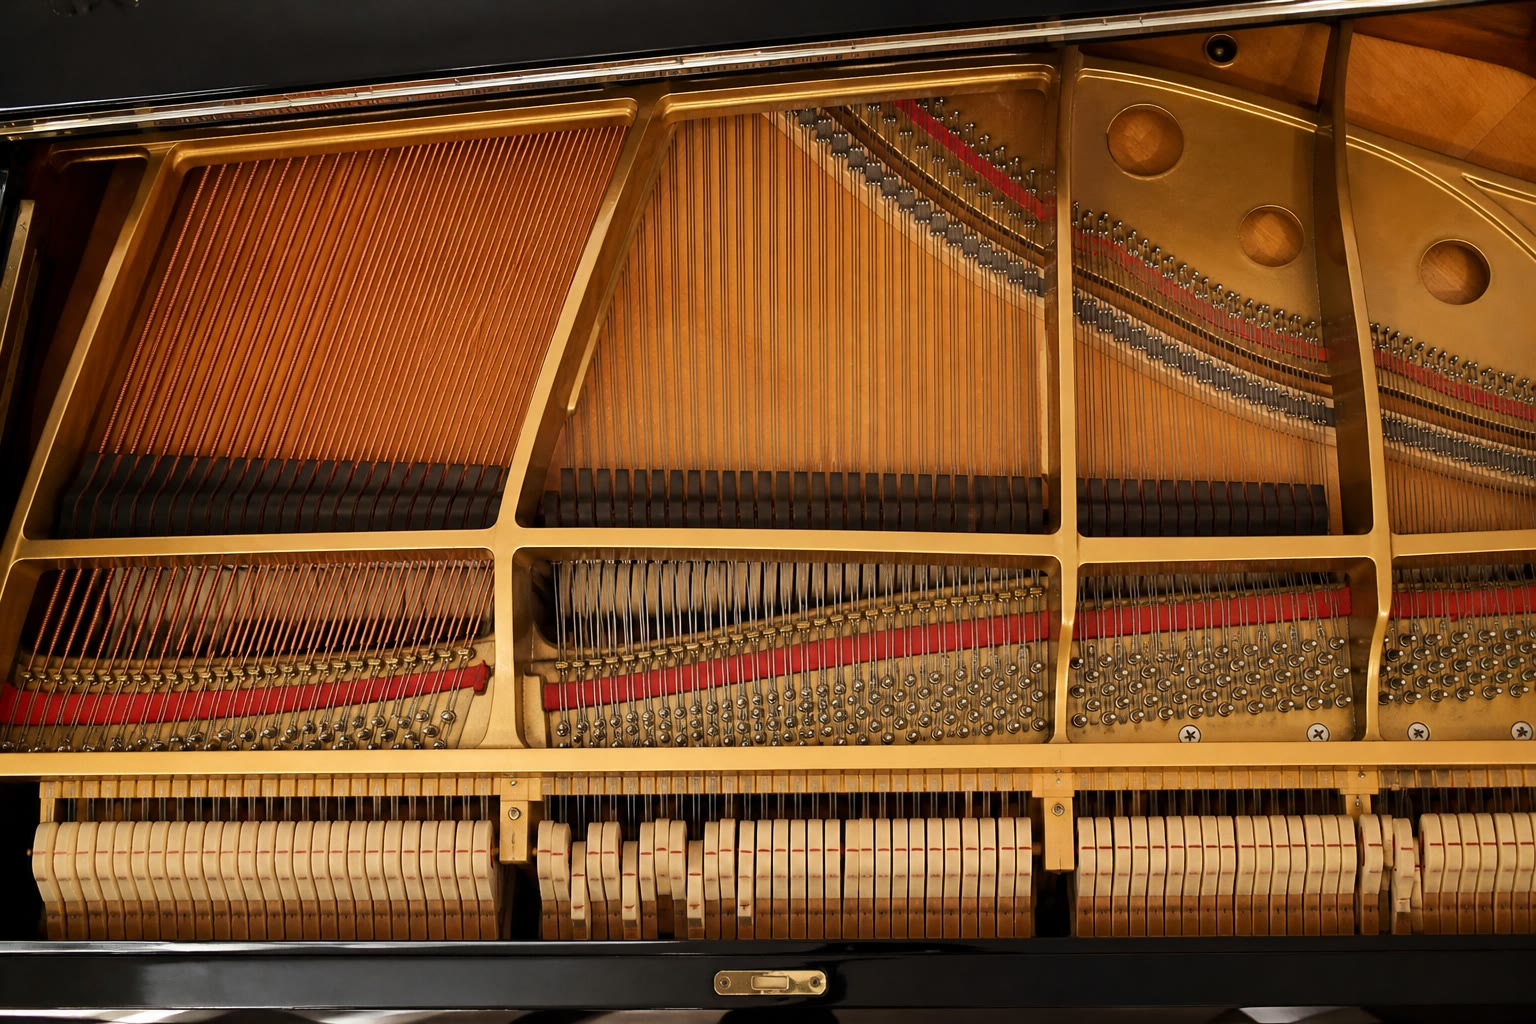
\includegraphics[width=0.58\linewidth]{images/book4/ai/b4-06-grand-piano-strings.jpg}

{\small 三角钢琴内部：约两百根长度与粗细各异的钢弦，每根通过张力调至基频 $c/2L$；低音弦缠绕铜丝以增加质量。}
\end{omfigure}

\section{问题：钢琴，从琴槌到音板}

\begin{problem}[{周末问题——拆解一根钢琴弦：其
张力与劲度，琴槌的敲击及其产生的谐音，
将能量泄漏到音板的琴桥，以及
一根传播同一方程的钢轨}]
\label{pb:b2:waves-on-strings:1}

\medskip
\noindent\textbf{第一部分——弦。}
钢琴的 A$_4$ 弦（\qty{440}{Hz}）：钢制，$E = \qty{200}{GPa}$，$\rho =
\qty{7800}{kg/m^3}$，直径 $d = \qty{1.0}{mm}$，发声长度 $L =
\qty{38}{cm}$。除低音外，每个音都由三根此类弦发出；钢琴共有
$230$ 根弦。
\begin{enumerate}
  \item 弦的线密度、波速和张力。
  \item 钢丝中的拉应力；钢丝在 \qty{2.0}{GPa} 时断裂：
        安全裕度，以及为何调音时最后一转
        最为危险。
  \item 估算琴架上的总张力，设所有弦
        的张力均相同。
  \item 最低音弦（A$_0$，\qty{27.5}{Hz}）长 \qty{1.9}{m}；若它
        是同一张力下的普通钢丝，需要多大的 $\mu$ 和
        多大的直径？实际上它是绕有铜丝的钢芯，
        请说明原因。
  \item A$_4$ 弦的模式：前八个谐音的频率；
        哪些与基音构成协和音程
        （八度、五度、四度、大三度），哪些不
        构成？
  \item 弦以基频振动，其振幅在波腹处为
        \qty{0.50}{mm}，求储存的能量（一个模式的能量
        为 $\tfrac14\mu L\omega^2A^2$）。
  \item 将基频写成两列行波之和，并给出
        它们的振幅以及各自传递的平均功率。
\end{enumerate}

\medskip
\noindent\textbf{第二部分——锤击。}
锤子在 $x_0 = L/8$ 处敲击弦，在 $t = 0$ 时，
使弦上一小段获得速度 $v_0$，
该段宽度为 $w$，位于 $x_0$ 附近，位移为零。
\begin{enumerate}[resume]
  \item 写出一般解 $y = \sum_nB_n\sin(n\pi x/L)\sin(\omega_nt)$，
        并利用正弦函数的正交性证明 $B_n =
        \dfrac{2}{L\omega_n}\int_0^L\dot y(x, 0)\sin\dfrac{n\pi x}L\,\dd x$。
  \item 对于窄的敲击（$w \ll L/n$），证明 $B_n \approx \dfrac{2v_0w}
        {L\omega_n}\sin\dfrac{n\pi x_0}{L}$。
  \item 当 $x_0 = L/8$ 时，哪些谐音缺失？钢琴制造者为什么
        在 $L/7$ 至 $L/8$ 附近敲击（见第 5 题）？
  \item 从行波图像描述运动：从被敲击点离开的是什么，
        两端发生什么，经过多长时间
        初始状态会再现？
  \item 实际的弦略有刚性：其模式为 $f_n = nf_1
        \sqrt{1 + Bn^2}$，其中 $B = \pi^3Ed^4/(64TL^2)$（在本阶段不加证明地承认）。计算
        $B$ 以及第八谐音的升高量，分别以百分比和
        音分表示（\qty{1}{cent} 对应频率比 $2^{1/1200}$）。
  \item 钢琴调音师为什么要“拉伸”八度（将高音
        略微调高）？
\end{enumerate}

\medskip
\noindent\textbf{第三部分——琴马与音板。}
弦跨过粘在音板上的琴马；音板在琴马处
表现得如同阻抗为 $Z_b = \qty{2000}{kg/s}$ 的弦。
\begin{enumerate}[resume]
  \item 求弦的阻抗 $Z_s$，以及
        琴马处的振幅反射系数。
  \item 每次反射时，传入音板的能量占波能量的
        比例。
  \item 求每秒在琴马处的反射次数；由此推出
        能量衰减的时间常数，以及声音降低
        \qty{60}{dB}（能量因子为 $10^6$）所需的时间。
  \item 求第 6 题中敲击后刚泄漏到音板中的功率，
        并与安静交谈的功率相比较，
        后者约为 \qty{1e-5}{W} 的声功率。
  \item 为什么单独的弦几乎听不见，音板
        对此做了什么？（考虑空气的阻抗
        $\rho c \approx \qty{400}{kg.m^{-2}.s^{-1}}$，从
        小面积对大面积的作用来看。）
  \item 抬起阻尼器后，A$_3$ 弦
        （\qty{220}{Hz}）在弹奏 A$_4$ 时开始发声：为什么？
  \item 钢琴制造者希望延长余音：$Z_b$ 应当
        增大还是减小？会损失什么？
\end{enumerate}

\medskip
\noindent\textbf{第四部分——钢轨。}
一根钢轨（$E = \qty{200}{GPa}$，$\rho = \qty{7800}{kg/m^3}$，截面积
        \qty{70}{cm^2}）。
\begin{enumerate}[resume]
  \item 求压缩波的速率；求火车的声音
        沿钢轨及空气传播 \qty{5}{km} 所需的时间。
  \item 锤击使一个压缩脉冲沿一段长 \qty{25}{m}、
        一端自由的钢轨传播：求回波所需的时间；回波是
        压缩还是稀疏？
  \item 超声 \qty{2}{MHz} 探头用于探测裂纹：求钢中的
        波长；求钢—空气裂纹处的振幅反射系数
        （空气阻抗 $\qty{400}{kg.m^{-2}.s^{-1}}$）；说明为什么细裂纹
        能被如此清楚地探测到。
  \item 地震：在岩石中，压缩（P）波的传播速率为
        \qty{6.0}{km/s}，剪切（S）波为 \qty{3.5}{km/s}。某台站
        记录到 S 波比 P 波晚 \qty{20}{s}：求震源的
        距离。
  \item 在一张表中汇总本题的五种波速
        （弦、钢轨、岩石 P 波、岩石 S 波、空气），并列出决定
        各自大小的劲度与惯性。
\end{enumerate}
\end{problem}
